\documentclass[a4paper,10pt]{article}
\usepackage[spanish]{babel}
\usepackage[utf8]{inputenc}
\usepackage{packages/caratula}
\usepackage{packages/algo2symb}
\usepackage{packages/newalgo}
\usepackage{packages/itef}
\usepackage{packages/boxedfile}
\usepackage{colortbl}
\usepackage{color}
\usepackage{multicol}
\usepackage{multirow}


\usepackage{footnote}
\makesavenoteenv{tabular}
\usepackage{amsmath}
\usepackage{amsthm}
\usepackage[pdftex]{graphicx}
\usepackage{makeidx}
\usepackage{textcomp}
\usepackage{fancyhdr}
\usepackage{subfigure}
\usepackage{lastpage}
\usepackage{listings}
\usepackage{hyperref}
\hypersetup{
    colorlinks=false,
    pdfborder={0 0 0},
}
\usepackage{alltt}
\usepackage{wasysym}
\usepackage{float}

\pagestyle{fancy}

\makeindex
\fancyhf{}
\fancyhead[LO]{Orga2, TP Final -- WxCam}
\fancyhead[RO]{\thepage~de \pageref{LastPage}}
\addtolength{\headwidth}{\marginparsep}
\addtolength{\headwidth}{\marginparwidth}
\addtolength{\headwidth}{\marginparsep}
\addtolength{\headwidth}{\marginparwidth}
\renewcommand{\headrulewidth}{0.5pt}

\usepackage[top=3cm,bottom=2cm,left=2cm,right=2cm]{geometry}

\definecolor{light-gray}{gray}{0.90}
\definecolor{dark-gray}{gray}{0.75}

\newcommand{\maximo}[2]{\max_{\;#1}\big(#2 \big)}
\newcommand{\nil}{\textbf{nil}}

\newcommand{\strongnewpage}{\newpage\mbox{} \newpage}
\newcommand{\comment}[1]{{\small{\emph{\textcolor{blue}{#1}}}}}
\newcommand{\complex}[1]{$\mathcal{O}(#1)$}

\newtheorem{prop}{Proposición}
\newtheorem{lema}{Lema}
\newtheorem{teorema}{Teorema}

\newfloat{codef}{ht}{codetemp}
\floatname{codef}{Código}


\lstloadlanguages{C++}
\lstnewenvironment{code}
	{\csname lst@SetFirstLabel\endcsname}
	{\csname lst@SaveFirstLabel\endcsname}
\lstset{
	language=C++, basicstyle=\small\ttfamily, keywordstyle=\slshape,
	emph=[1]{tipo,usa}, emphstyle={[1]\sffamily\bfseries},
	morekeywords={tint,forn,forsn},
	basewidth={0.47em,0.40em},
	columns=fixed, fontadjust, resetmargins, xrightmargin=5pt, xleftmargin=15pt,
	flexiblecolumns=false, tabsize=2, breaklines,	breakatwhitespace=false, extendedchars=true,
	numbers=left, numberstyle=\tiny, stepnumber=1, numbersep=9pt,
	frame=l, framesep=3pt,
}

\begin{document}

    \materia{Organizaci\'on del Computador II}

    \titulo{Trabajo Pr\'actico Final}

    

	\integrante{Adri\'an Bonaccini}{207/04}{adrian.bonaccini@gmail.com}
    \integrante{Sebastian Galimberti}{763/04}{galimba@gmail.com}
	
  \maketitle
  \tableofcontents
  \newpage
  \section{Introducción}

Luego de instalar una webcam, siempre es bueno probar su funcionamiento. Para tal fin los diseñadores de Apple incluyen PhotoBooth en sus instalaciones de OSX. PhotoBooth permite aplicar una gran variedad de filtros y junto con su calidad de imagen hacen de este software una aplicaci\'on de entretenimiento

Generalmente, los usuarios de Microsoft cuentan con una opci\'on clara a la hora de testear su webcam, dado que cada webcam viene con sus drivers y su software propietario para administrarla.

Sin embargo, los usuarios de sistemas operativos basados en Linux y BSD no cuentan con estas ventajas. Son pocas las empresas que diseñan webcams e incluyen drivers para Linux, aunque existen drivers gen\'ericos (por ejemplo qc-usb y libv4l). A la hora de interactuar con la webcam, los usuarios Linux recurren a la comunidad en busca de un software acorde a sus necesidades. Si bien existen soluciones implementadas (Camorama, Cheese, WxCam, entre otras) a menudo no vienen inclu\'idas por defecto en las distribuciones mas populares de Linux y aun as\'i, los efectos de video disponibles son limitados y lentos.

La finalidad de este trabajo es desarrollar un conjunto de filtros para im\'agenes, aplicables al video de captura de una webcam. Para tal fin, consideramos las alternativas Open Source disponibles en la comunidad. De las aplicaciones disponibles, decidimos encarar este proyecto utilizando WxCam por su simplicidad y versatilidad.

  \newpage
  \section{WxCam}

\subsection{El proyecto}
WxCam es una aplicaci\'on para Linux. El software interact\'ua con la webcam a trav\'es del driver v4l-1 o v4l-2, que es uno de los mas utilizados. El proyecto est\'a activo (el \'ultimo release - v1.01 - fue hace unos pocos meses) y cuenta con dos main-developers y aproximadamente 15 contribuyentes. El programa soporta capturas de video, de im\'agenes y la aplicaci\'on de 10 filtros de im\'agenes, programados en C++ sin la utilizaci\'on de librer\'ias espec\'ificas, lo que los hace lentos para la aplicaci\'on en tiempo real.

El presente trabajo busca suplir esta falta reimplementando estos filtros mediante instrucciones SIMD en lenguaje ensamblador para la arquitectura amd64. Asimismo buscamos que el proyecto sea mas atractivo al usuario final, por ende inclu\'imos una serie de filtros avanzados que ser\'an programados bajo la misma premisa de cuidado de la performance. Estos \'ultimos son ideados con el fin de transformar la herramienta en un programa de entretenimiento capaz de crear im\'agenes y videos divertidos.

\subsection{Plataforma}
Los desarrolladores del proyecto optaron por programar utilizando NetBeans como IDE, lo cual nos fuerza a utilizar el mismo software para implementar las mejoras. Decidimos utilizar la arquitectura amd64 debido a su amplio uso actual en PCs. Para explotar el potencial, trabajamos sobre Linux (K)Ubuntu y Mac OSX utilizando las \'ultimas versiones de SSE. Nuestro compilador assembler es NASM dada su mejor integraci\'on con NetBeans.

\subsection{Filtros}
WxCam tiene una implementaci\'on en C++ de varios filtros. Los algoritmos son simples y no estan optimizados (con la excepci\'on del par\'ametro -O2 que utiliza el IDE para compilar). Para realizar el presente trabajo evaluamos la lista de filtros del proyecto Gimp, tambi\'en Open Source, y decidimos implementar los siguientes efectos visuales: \\
\begin{itemize}
\item[1] Vertical Mirror: cada pixel se transporta entero de acuerdo a la distancia axial al centro de la imagen,
\item[2] Negative: calcula el color inverso para cada pixel,
\item[3] Stretch: zoom X2,
\item[4] Edge: calcula un Sobel con caracterizaci\'on de colores,
\item[5] Bona: filtro por distancia de colores espec\'ificos (ie. el rojo) y en caso de ser cercano se lo deja intacto,
\item[5] Pixelate: distorsiona la imagen exagerando el pixelado,
\item[6] Instagram: el efecto del filtro simula que la imagen fue tomada por una camara antigua,
\item[7] Monochrome: pasaje a blanco/negro,
\item[8] Channel: filtrado por canales (R, G o B),
\item[9] Median: reducci\'on de ru\'ido a trav\'es del c\'alculo de promedios en la vecindad,
\end{itemize}

  \clearpage
  \section{Desarrollo}
  
\subsection{General}

\subsubsection{Vertical Mirror}

Copia la primera parte de la imagen en la segunda parte, espej\'andola con respecto a la vertical. Cada pixel se transporta entero de acuerdo a la distancia que tiene a la l\'inea central de la imagen. Para cada pixel $p$ se eval\'ua lo siguiente:\\
\begin{center}
$Posicion(p') = ancho - Posicion (p)$
\end{center}
\subsubsection*{Pseudo-C\'odigo}
\begin{verbatim}
para cada fila de 0 a altura-1
     para cada pixel de 0 a ancho/2 sobre esta fila
          copiar el pixel de pos_P en: ancho - pos_P
\end{verbatim}
\subsubsection*{Ejemplo}
\begin{center}
  \begin{figure}[H]
  
\includegraphics[scale=0.60]{imgs/vmirr.png}
  \end{figure}  
\end{center}

\subsubsection{Negative}

Este filtro invierte los colores en cada pixel de la imagen. Para invertir un pixel se realiza la diferencia con 255 de cada canal.\footnote{http://es.wikipedia.org/wiki/Inversion\_(imagen)}
Dado un pixel $p$:\\

\begin{center}

Neg(R) = 255 - R

Neg(G) = 255 - G

Neg(B) = 255 - B
 
\end{center}
\subsubsection*{Pseudo-C\'odigo}
\begin{verbatim}
para cada fila de 0 a altura-1
     para cada pixel de 0 a ancho sobre esta fila
          en la pos_P del pixel_P calcular: - pixel_P
\end{verbatim}
\subsubsection*{Ejemplo}
\begin{center}
  \begin{figure}[H]
  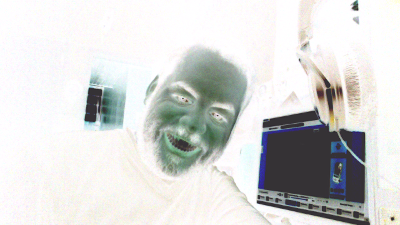
\includegraphics[scale=0.60]{imgs/neg.png}
 % \caption{}
  \end{figure}  
\end{center}

\subsubsection{Stretch (zoom x2)}

Transforma la imagen de forma tal que cada pixel $p$ se copia 3 veces en las posiciones de sus vecinos a izquierda, abajo y diagonal, generando una imagen resultado que es equivalente a hacer zoom sobre el primer cuadrante de la imagen original.\footnote{http://en.wikipedia.org/wiki/Nearest-neighbor\_interpolation}
\subsubsection*{Pseudo-C\'odigo}
\begin{verbatim}
para cada fila de 0 a altura/2
     para cada pixel de 0 a ancho/2 sobre esta fila
          en la pos_P del pixel_P copiar pixel_P
          copiar pixel_P a la derecha, abajo y diagonal
\end{verbatim}
\subsubsection*{Ejemplo}
\begin{center}
  \begin{figure}[H]
  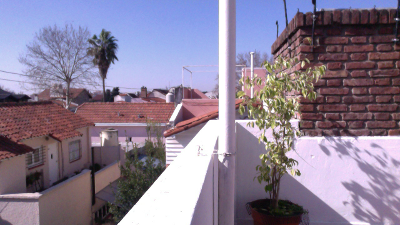
\includegraphics[scale=0.60]{imgs/stretch1.png}
  \end{figure}  
  \begin{figure}[H]
  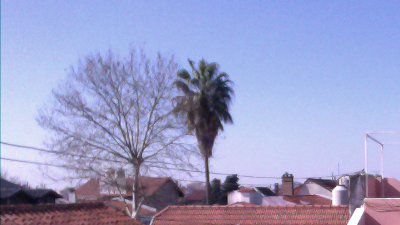
\includegraphics[scale=0.60]{imgs/stretch2.png}
  \end{figure}  
\end{center}  

\subsubsection{Edge (Sobel + colores)}

Este filtro detecta los bordes utilizando el algoritmo Sobel. Se examina cada pixel de la imagen, para cada uno se multiplica el valor de este pixel y los valores de los 8 circundantes por el valor correspondiente de la matriz. El pixel del centro de la matriz regula su valor de acuerdo al valor resultante de la operaci\'on. La dificultad est\'a puesta en aprovechar las bondades de las instrucciones SIMD y sus capacidades para trabajar en grandes lotes.\footnote{$http://en.wikipedia.org/wiki/Sobel_operator)$} \\
La matriz de convolucion X es:
\begin{center}
$\begin{bmatrix}
  +1 & 0 & -1 \\
  +2 & 0 & -2 \\
  +1 & 0 & -1
 \end{bmatrix}$
 \end{center}
La matriz de convolucion Y es:
\\
\begin{center}
$\begin{bmatrix}
  +1 & +2 & +1 \\
  0 & 0 & 0 \\
  -1 & -2 & -1
 \end{bmatrix}
$\end{center}

\subsubsection*{Pseudo-C\'odigo}
\begin{verbatim}

se hace una pasada para calcular las derivadas parciales en X
se hace otra pasada para calcular las derivadas parciales en Y
    se genera el gradiente de (X,Y) y se guarda en cada pixel
\end{verbatim}
\subsubsection*{Ejemplo}
\begin{center}
  \begin{figure}[H]
  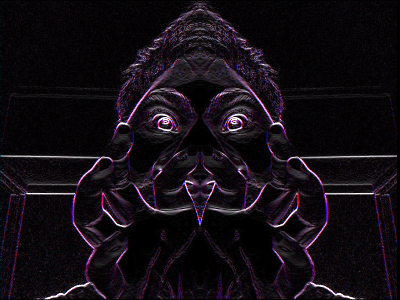
\includegraphics[scale=0.60]{imgs/sobel.png}
  \end{figure}  
\end{center}  

\subsubsection{Bona (distancia a un color)}

El algoritmo genera un filtro y una conversi\'on en la imagen. Son utilizados dos par\'ametros de entrada: color y tamaño de la ventana. Por cuestiones est\'eticas se decidi\'o utilizar el rojo como color par\'ametro y la medida de la ventana se acomoda de acuerdo al nivel de apertura del obturador e ISO de la c\'amara. En muchas webcams estos par\'ametros son manejados por el driver mismo, quedando el threshold como \'unico par\'ametro para obtener el efecto deseado.

Respecto de la l\'ogica de la rutina, se mide la distancia geom\'etrica de cada pixel al color par\'ametro y, en caso de ser cercano, se deja como se encontraba. En caso de tener una distancia mayor a la sugerida por el tamaño de ventana, se monocromatiza el pixel. El efecto deseado destaca en la imagen el color par\'ametro elegido.\footnote{http://stackoverflow.com/questions/9018016/how-to-compare-two-colors}

\subsubsection*{Pseudo-C\'odigo}
\begin{verbatim}
para cada pixel p de la imagen:
    si la distancia de colores entre p y rojo es mayor a la ventana
        se monocromatiza el pixel con el algoritmo (R+2G+B)/4
\end{verbatim}
\subsubsection*{Ejemplo}
\begin{center}
  \begin{figure}[H]
  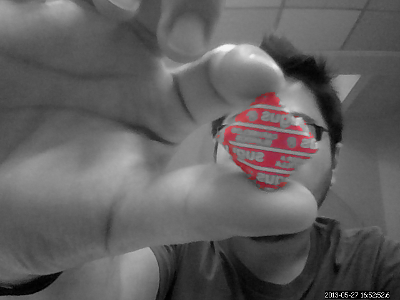
\includegraphics[scale=0.60]{imgs/bona.png}
  \end{figure}  
\end{center}  

\subsubsection{Pixelate}

Como su nombre lo indica, el algoritmo pixela la imagen mediante la p\'erdida de informaci\'on de la misma. Para ello, construye una matriz cuadrada de tamaño param\'etrico y replica la informaci\'on del pixel (0;0) en el resto de los p\'ixeles de la matriz. La imagen resultante simula haber perdido calidad y se asemeja a la de los viejos personajes de los juegos de 8 bits. La complejidad del algoritmo est\'a ubicada en hacerlo param\'etrico al tamaño de la matriz y que, a pesar de que el tamaño sea variable, se siguieran utilizando las bondades del procesamiento en paralelo que proveen las instrucciones SIMD.\footnote{http://en.wikipedia.org/wiki/Pixelation}

\subsubsection*{Pseudo-C\'odigo}
\begin{verbatim}
para cada sub-matriz de n x n pixels
    se toma el valor de (0,0) y se lo copia en el resto de las posiciones de la sub-matriz
\end{verbatim}

\subsubsection*{Ejemplo}
\begin{center}
  \begin{figure}[H]
  
\includegraphics[scale=0.60]{imgs/pix.png}
 % \caption{}
  \end{figure}  
\end{center}

\subsubsection{Instagram}

El efecto que propone el filtro es la simulaci\'on de que la imagen fue tomada por una camara antigua. El objetivo es darle un aspecto tostado al video. Este mismo efecto fue popularizo por la red social Instagram y es la acumulaci\'on de otros efectos sobre la misma imagen. Para lograrlo se le baja el brillo, se le sube el contraste y se ruboriza la imagen. La ruborizaci\'on de la imagen la resolvimos ubicando a los p\'ixeles en dos grupos seg\'un su distancia al color negro (\#0,0,0), los que mas distancia ten\'ian eran ruborizados con menos fuerza (10h) y los dem\'as con 16h para obtener el efecto final tostado y que no se rompiera la continuidad con la diferencia de color.\footnote{http://net.tutsplus.com/tutorials/php/create-instagram-filters-with-php/}

\subsubsection*{Pseudo-C\'odigo}
\begin{verbatim}
Para cada pixel de la imagen:
    si dista del negro mas que la ventana
        se le suman 10h a la componente R
    si la distancia no es suficiente
        se le suman 16h a la componente R
Luego, para cada pixel de la imagen:
    se reduce el brillo, restando 40 a todas las componentes R, G y B
    se aumenta el contraste un 25%
\end{verbatim}

\subsubsection*{Ejemplo}
\begin{center}
  \begin{figure}[H]
  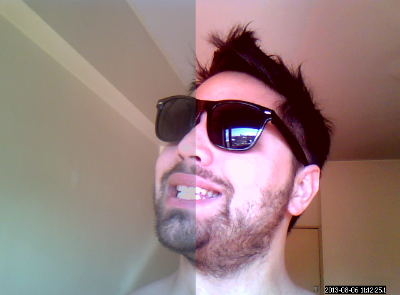
\includegraphics[scale=0.60]{imgs/insta.png}
 % \caption{}
  \end{figure}  
\end{center}

\subsubsection{Monochrome}

Pasa la imagen a escala de grises.\footnote{http://www.tannerhelland.com/3643/grayscale-image-algorithm-vb6/} Para monocromatizar cada pixel $p$, se considera la cuenta:
\begin{center}
$ (R + 2G + B ) * 1/4 $
\end{center}
\subsubsection*{Pseudo-C\'odigo}
\begin{verbatim}
para cada pixel p en la imagen:
     el valor de R, G y B se pisa con el resultado de la cuenta: (R + 2G + B ) * 1/4
\end{verbatim}

\subsubsection*{Ejemplo}
\begin{center}
  \begin{figure}[H]
  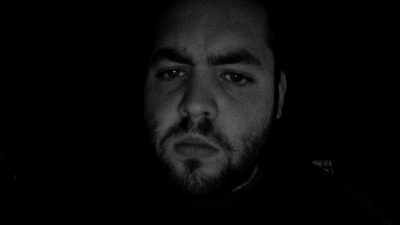
\includegraphics[scale=0.60]{imgs/mono.png}
  \end{figure}  
\end{center}  

\subsubsection{Channel}

Este filtro considera un \'unico canal (el R, G o B) y filtra los otros dos. La imagen resultante es monocrom\'atica roja-negro, verde-negro o azul-negro.
\subsubsection*{Pseudo-C\'odigo(Red)}
\begin{verbatim}
para cada pixel p en la imagen:
    el valor de G y B se pisa con 0   
\end{verbatim}

\subsubsection*{Ejemplo}
\begin{center}
  \begin{figure}[H]
  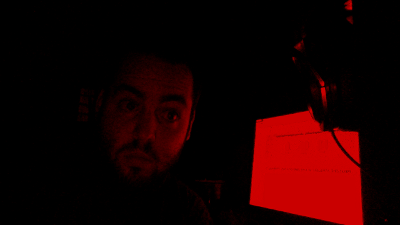
\includegraphics[scale=0.60]{imgs/chan.png}
  \end{figure}  
\end{center}  

\subsubsection{Median}

Dado un pixel $p$, el filtro calcula el promedio de cada vecindad. Las vecindades son de 5x5 pixels y el efecto resultante produce una disminuci\'on del ruido en la imagen. Como efectos colaterales, se pierde un poco de brillo y detalle en la imagen.\footnote{$http://en.wikipedia.org/wiki/Median_filter$}
\subsubsection*{Pseudo-C\'odigo}
\begin{verbatim}
para cada fila entre 2 y altura - 2:
    para cada columna entre 2 y ancho - 2:
        para cada pixel p:
            se calcula el promedio R, G y B de todos los 8 vecinos
            se pisa p con el promedio R, G y B de la vecindad
\end{verbatim}

\subsubsection*{Ejemplo}
\begin{center}
  \begin{figure}[H]
  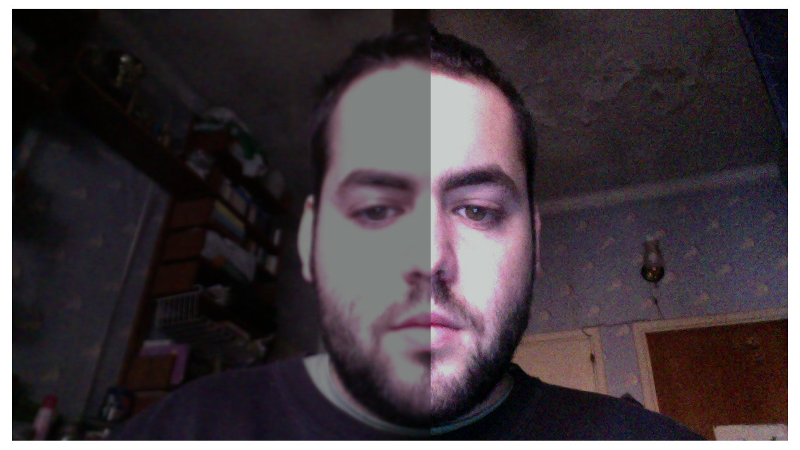
\includegraphics[scale=0.40]{imgs/median.png}
  \end{figure}  
\end{center}  

  \newpage
  \section{Resultados}
 Los filtros se testearon tanto en Linux como en OSX, utilizando webcams de definici\'on $640 x 480$ tanto como HD-720. Las webcams tienen una limitaci\'on promedio de 20 FPS. La comparaci\'on se realiza sin par\'ametros de optimizaci\'on y con -03. Para analizar la velocidad y medir los tiempos de respuesta de las diferentes implementaciones no alcanza con mirar los FPS, as\'i que decidimos utilizar el TSC. Para tal fin generamos la siguiente rutina que es llamada antes de cada algoritmo:
 \begin{verbatim}
 static __inline__ unsigned long rdtsc(void)
{
   //unsigned long long int x;
   unsigned a, d;

   __asm__ volatile("rdtsc" : "=a" (a), "=d" (d));

   return (((unsigned long)a) | (unsigned long)d >> 32);
}
 \end{verbatim}
 En la siguiente tabla se ven las diferencias (medidas en cantidad de ciclos promedio) entre los algoritmos implementados en C++ y assembler (con y sin optimizaciones de compilador).
 Para calcular el promedio de ciclos por aplicacion del algoritmo se ejecuta el programa, se activa el filtro y se mide durante 30 segundos la diferencia de RDTSC entre el inicio y final de cada llamada al filtro. Luego se promedian todos los datos.

\begin{center}
    \begin{tabular}{ | l | l | l | p{5cm} |}
    \hline
    Filtro & gcc & gcc -O3 & SSE \\ \hline
    Monochrome & 4244864  & 3463785 & 4244864  \\ \hline
    Negative & 16895274 & 755973 & 866218  \\ \hline
    Sobel & 225153350 & 22634335 & 15596374  \\ \hline
    Median & 3414938448 & 1786994543 & 13632900  \\ \hline
    \end{tabular}
$ $ \\ \textit{Los datos est\'an expresados en cantidad de tics del CPU de acuerdo al TSC}
\end{center}
  \section{Discusi\'on}

\subsection{Problemas encontrados}
\begin{itemize}

\item A lo largo del proceso de selecci\'on de los filtros consideramos como prioritario aportar a la comunidad Open Source una aplicaci\'on con las herramientas necesarias para que sea entretenida y \'util. Dicho esto, descartamos algoritmos que cubrieran el mismo efecto (ie. para reconocimiento de bordes utilizamos Sobel, descartando Laplacian y Canny).
\item Nuestra intenci\'on fue implementar (en assembler SIMD) filtros similares a los de la aplicaci\'on PhotoBooth de OSX. Algunos de estos filtros fueron descartados por la naturaleza de los algoritmos. Un caso no abordado fue el efecto conocido como Swirl, que utiliza cambio de coordenadas para los pixeles, lo que imposibilita el aprovechamiento de las instrucciones SIMD en el algoritmo.
\item Luego de programar los algoritmos Pixelar y Median nos percatamos que, aunque el filtro estaba siendo bien aplicado, el efecto logrado no tenia la intensidad deseada: El pixelado era muy peque\~no y la reducci\'on de ruido era muy pobre. Decidimos ampliar el algoritmo para recibir un parametro m\'as, que contemple el tama\~no de la ventana de pixels y la cantidad de aplicaciones de promedio para reducci\'on de ruido.


\end{itemize}

\subsection{Performance de los filtros}
Luego de analizar los resultados, podemos afirmar que la performance de cada uno de los filtros que optimizamos ha mejorado considerablemente con respecto a la compilaci\'on sin par\'ametros de optimizaci\'on. Con respecto a la compilaci\'on optimizada (con el parametro -O3), los algoritmos simples (monocromatizar, negativo) parecen mejorar considerablemente (con una ganancia de 15 porciento de velocidad con respecto a nuestra implementaci\'on SSE). En la pr\'actica, vemos que el rendimiento de los filtros implementados con SSE es el deseado, sin p\'erdida considerable de FPS en la aplicaci\'on (incluso considerando la superposici\'on de filtros). Con respecto a los filtros programados en C++, se nos present\'o el problema de que algunos algoritmos son tan lentos que, incluso con optimizaciones -O3 no llegan a ser utilizables (Median, Sharpen). Esto se debe a la naturaleza del algoritmo.

\subsection{Las condiciones de testing}
Dado que nuestros equipos a lo sumo pueden capturar im\'agenes de 720p a 20 frames por segundo, queda abierta la posibilidad de que estos algoritmos escalen a una performance diferente cuando estemos utilizando im\'agenes full HD (de 1080p a 50 frames por segundo). A futuro y con fines acad\'emicos, ser\'ia interesante explorar \'esta posibilidad para utilizar webcams que cuenten con mejor calidad de imagen y analizar nuevamente el comportamiento de estas optimizaciones.\\


  \newpage
   \section{Referencias}

\begin{itemize}
\item[1] $http://docs.gimp.org/en/filters.html$
\item[2] $http://git.gnome.org/browse/gimp/tree/plug-ins/common$
\item[3] $http://en.wikipedia.org/wiki/Image_scaling$
\item[4] $http://www.steves-digicams.com/knowledge-center/brightness-contrast-saturation-and-sharpness.html$
\item[5] $http://www.dfstudios.co.uk/articles/image-processing-algorithms-part-5/$
\item[6] $http://www.johndcook.com/blog/2009/08/24/algorithms-convert-color-grayscale/$
\item[7] $http://www.codeproject.com/Articles/3419/Image-Processing-for-Dummies-with-C-and-GDI-Part-5$
\item[8] $http://www.jhlabs.com/ip/filters/index.html$
\item[9] $http://stackoverflow.com/questions/11165564/edge-detectors-for-rgb-images$
\item[10] $http://www.cambridgeincolour.com/tutorials/image-interpolation.htm$
\item[11] $http://net.tutsplus.com/tutorials/php/create-instagram-filters-with-php/$
\item[12] $http://softpixel.com/~cwright/programming/simd/sse.php$
\item[13] $http://en.wikipedia.org/wiki/Streaming_SIMD_Extensions$
\item[14] $http://support.amd.com/us/Processor_TechDocs/43479.pdf$
\item[15] $http://www.programming-techniques.com/2013/02/median-filter-using-c-and-opencv-image.html$
\item[16] $http://en.wikipedia.org/wiki/Color_difference$
\item[17] $http://stackoverflow.com/questions/9018016/how-to-compare-two-colors$
\item[18] $http://stackoverflow.com/questions/225548/resources-for-image-distortion-algorithms$
\item[19] $http://docs.opencv.org/doc/tutorials/core/basic_linear_transform/basic_linear_transform.html$
\item[20] $http://es.wikipedia.org/wiki/Inversion\_(imagen)$
\item[21] $http://en.wikipedia.org/wiki/Median_filter$
\item[22] $http://www.tannerhelland.com/3643/grayscale-image-algorithm-vb6/$

\end{itemize}
   \newpage
   \section{Ap\'endice}
\subsection{C\'odigo SSE}
\subsubsection{Vertical Mirror}
\begin{verbatim}
global verticalMirror_asm ;verticalMirror_asm(unsigned char* frame, int size, int width, height);
section .data

shuffle: dd 0x0E0D0C0F, 0x060B0A09, 0x04030807, 0x02010005

section .text

verticalMirror_asm:
        ; los parametros son pasados asi:
        ;	rdi= char* frame
        ;	rsi= int size
        ;       rdx= int width
        ;       rcx= int height !!!
        ;
	push rbp	;     reservo
	mov rbp,rsp	;       la
	push rbx	;      pila
	push r12	;        y
	push r13	;      guardo
	push r14	;    registros
	push r15	;   (...)

	;;;;;;;;;; Aca comienza la funcion ;;;;;;;;
        mov r12, rdx
        sar r12, 1      ; r12 = ancho/2
        ;lea r15, [rdi + rsi - 1] ; r15 = (img+size) para controlar el final
        lea r15, [rdi + rsi]; r15 = (img+size) para controlar el final
        xor rbx, rbx
        
.ciclo_largo:
        
        .ciclo_corto:
            pxor xmm1, xmm1
            lea r14, [rdi + rbx] ; cargo la dir. de memoria que quiero levantar
            movdqu xmm1, [r14]	; xmm1 = aR|aG|aB|bR|...|eB|fR = (5 pixels abcde + 1 byte de f)	
            ;lea r13, [r14 + r12] ; cargo el destino
            lea r13, [rdi+rdx]  ; r13 = primer byte de la siguiente linea
            sub r13, rbx        ; r13 = lugar donde termina el cacho de imagen a mover
            sub r13, 16         ; r13 = destino a mover la imagen
            ; ahora tengo que dar vuelta los pixels
            ; uso la mascara
            ; NOTA: acomodar para usar 15 bytes, por el orden inverso de pixels
            movdqu xmm2, [shuffle]
            pshufb xmm1, xmm2
                       
            
            ; devuelvo a memoria la imagen espejada
            movdqu [r13], xmm1  ; guardo los datos
            add rbx, 15 ; aumento el contador
            cmp rbx, r12    ; comparo si llegue a media pantalla levantando
            jne .ciclo_corto
            
            add rdi, rdx    ; paso a la siguiente fila
            xor rbx, rbx    ; limpio el contador
        cmp rdi, r15    ; comparo si llegue al final de la imagen
        jl .ciclo_largo

	pop r15		;   restauro
	pop r14		;     los
	pop r13		;   registros
	pop r12		;     por
	pop rbx		; convencion C
	pop rbp		;

ret
\end{verbatim}
\subsubsection{Negative}
\begin{verbatim}
global negative_asm ;negative_asm(unsigned char* frame, int size);
section .data

allF: db 0xFF, 0xFF, 0xFF, 0xFF, 0xFF, 0xFF, 0xFF, 0xFF, 0xFF, 0xFF, 0xFF, 0xFF, 0xFF, 0xFF, 0xFF, 0xFF

section .text

negative_asm:
        ; los parametros son pasados asi:
        ;	rdi= char* frame
        ;	rsi= int size
        ;
	push rbp	;     reservo
	mov rbp,rsp	;       la
	push rbx	;      pila
	push r12	;        y
	push r13	;      guardo
	push r14	;    registros
	push r15	;   (...)

	;;;;;;;;;; Aca comienza la funcion ;;;;;;;;
	xor rcx, rcx	; limpio el reg ;;;;;;;;;;;;;;;;;; CREO Q NO HACE FALTA
	mov rcx, rsi	; rcx <- size
	sar rcx, 4	    ; dividimos xq procesamos de a 16 bytes/canales
        
.ciclo:
    ; cargo los pixels en el registro
    movdqu xmm1, [rdi]	; xmm1 = aR|aG|aB|bR|...|eB|fR = (5 pixels abcde + 1 byte de f)	
    movdqu xmm2, [allF]
    psubsb xmm2, xmm1	; calculo el negativo complemento a dos
    movdqu [rdi], xmm2	; lo devuelvo al buffer
    add rdi, 16 	; avanzo el puntero
  loop .ciclo

	pop r15		;   restauro
	pop r14		;     los
	pop r13		;   registros
	pop r12		;     por
	pop rbx		; convencion C
	pop rbp		;

ret


\end{verbatim}
\subsubsection{Stretch}
\begin{verbatim}
;stretch_asm(unsigned char* frame, unsigned char* dst, int height, int width, int size);
global stretch_asm

section .rodata
ALIGN 16
lastOff:     dd 0xFFFFFFFF, 0xFFFFFFFF, 0xFFFFFFFF, 0x00FFFFFF
sinMedio: db 0xFF, 0xFF, 0xFF, 0xFF, 0xFF, 0xFF, 0x00, 0x00, 0x00, 0xFF, 0xFF, 0xFF, 0xFF, 0xFF, 0xFF, 0xFF
soloMedio: db 0x00, 0x00, 0x00, 0x00, 0x00, 0x00, 0xFF, 0xFF, 0xFF, 0x00, 0x00, 0x00, 0x00, 0x00, 0x00, 0x00
shuffle_1:   dd 0x00020100, 0x04030201, 0x05040305, 0xFFFFFFFF 

section .text

stretch_asm:
        ; los parametros son pasados asi:
        ;	rdi= char* src
        ;	rsi= char* dst
        ;       rdx= int height
        ;       rcx= int width en pixels
        ;       r8 = int size
	push rbp	;     reservo
	mov rbp,rsp	;       la
	push rbx	;      pila
	push r12	;        y
	push r13	;      guardo
	push r14	;    registros
	push r15	;   (...)

	;;;;;;;;;; Aca comienza la funcion ;;;;;;;;
        mov r8, rdi     ; r8 = frame
        mov r9, rsi     ; r9 = dest
        
        
        mov r14, rcx    ; voy a calcular el ancho de src en bytes
        add r14, rcx
        add r14, rcx    ; r14 = 3 * rcx
        mov rcx, r14    ; rcx = width en bytes
        sar r14, 1      ; r14 = ancho inicial de src en bytes
        mov r11, r14
        
        mov r10, rdx    ; r10 = alto de src en lineas
        sar r10, 1
        movdqa xmm0, [shuffle_1]
cicloLasFilas:
        sub r10, 1        ; correccion de emi, tengo que estirar copiando dos lineas
    cicloLasColumnas:        
        sub r11, 6      ; r11= cantidad de bytes restantes en la fila actual
        mov r12, r8     ; puntero a la linea actual en src
        mov r13, r9     ; puntero a la linea actual en dst
        ;;;;;
        movdqu xmm1, [r12]
        pshufb xmm1, xmm0
        movdqu [r13], xmm1
        movdqu [r13 + rcx], xmm1
        ;;;;;;
        add r8, 6
        add r9, 12
    cmp r11, 0
    jg cicloLasColumnas
        ;
        add r8, r14; media fila en src
        add r9, rcx


        mov r11, r14    ; restauro el contador de columnas
    cmp r10, 0      ; si todavia me faltan filas por recorrer
    jg cicloLasFilas

.end:

	pop r15		;   restauro
	pop r14		;     los
	pop r13		;   registros
	pop r12		;     por
	pop rbx		; convencion C
	pop rbp		;

ret

\end{verbatim}
\subsubsection{Edge}
\begin{verbatim}
;void edge_asm(unsigned char* src, unsigned char* dst, int height, int width);

%include "src/globales.mac";

global edge_asm
section .text

section .rodata
    unos:       dd 0xFFFFFFFF, 0xFFFFFFFF, 0xFFFFFFFF, 0xFFFFFFFF
    ceros:      dd 0x00000000, 0x00000000, 0x00000000, 0x00000000
    mask_255:   dd 0x00FF00FF, 0x00FF00FF, 0x00FF00FF, 0x00FF00FF

    ;Parameters
    ;rdi = char* source
    ;rsi = char* destiny
    ;rdx = int height
    ;rcx = int width
edge_asm:
    begin_convencion_C
	;;;;;;;;;; Aca comienza la funcion ;;;;;;;;
    inicializo_variables:
    mov r8, rdi         ; r8 = fuente
    mov r9, rsi         ; r9 = destino
    mov r10, rdx        ; r10 = alto
    mov r11, rcx        ; r11 = ancho en px
    add r11, rcx        ; http://goo.gl/XSAlJ
    add r11, rcx        ; r11 = ancho en bytes
    mov rcx, r10        ; ecx = contador de filas / alto

    ciclo_filas:
    mov rdx, r11        ; edx = contador de columnas / ancho
    ciclo_columnas:
    cmp rcx, r10
    jne sigue_1
    jmp pintar_negro    ; si estoy en la primera fila
    sigue_1:
    mov rax, r11
    sub rax, 3
    cmp rdx, rax
    jle sigue_2
    jmp pintar_negro    ; si estoy en la primera columna
    sigue_2:
    cmp rcx, 1
    jne sigue_3
    jmp pintar_negro    ; si estoy en la última fila
    sigue_3:
    cmp rdx, 1
    jne simd_sobel_X
    jmp pintar_negro    ; si estoy en la última columna
    simd_sobel_X:
    cmp rdx, 10         ; si tengo aún 10 bytes por levantar
    jg continuar_2
    jmp pintar_negro
    continuar_2:
    pxor XMM0, XMM0         ; limpio XMM0
    pxor XMM5, XMM5         ; resultados parciales parte ALTA
    pxor XMM6, XMM6         ; resultados parciales parte BAJA
    movdqu XMM7, [ceros]
    ; 1ra FILA
    sub r8, r11             ; subo el puntero una fila (lectura horizontal)
    movdqu XMM1, [r8-3]     ; leo desde el pixel anterior
    movdqu XMM2, [r8+3]     ; leo desde el pixel siguiente
    movdqu XMM3, XMM1
    movdqu XMM4, XMM2
    punpckhbw XMM3, XMM7    ; desempaqueto parte ALTA de XMM1
    punpckhbw XMM4, XMM7    ; desempaqueto parte ALTA de XMM2
    psubsw XMM5, XMM3       ; XMM5 parte alta (-1)
    paddsw XMM5, XMM4       ; XMM5 parte alta (+1)
    movdqu XMM3, XMM1
    movdqu XMM4, XMM2
    punpcklbw XMM3, XMM7    ; desempaqueto parte BAJA de XMM1
    punpcklbw XMM4, XMM7    ; desempaqueto parte BAJA de XMM2
    psubsw XMM6, XMM3       ; XMM6 parte baja (-1)
    paddsw XMM6, XMM4       ; XMM6 parte baja (+1)
    add r8, r11             ; vuelvo el puntero a su posición
    ; 2da FILA
    movdqu XMM1, [r8-3]     ; leo desde el pixel anterior
    movdqu XMM2, [r8+3]     ; leo desde el pixel siguiente
    movdqu XMM3, XMM1
    movdqu XMM4, XMM2
    punpckhbw XMM3, XMM7
    punpckhbw XMM4, XMM7
    psubsw XMM5, XMM3
    psubsw XMM5, XMM3
    paddsw XMM5, XMM4
    paddsw XMM5, XMM4
    movdqu XMM3, XMM1
    movdqu XMM4, XMM2
    punpcklbw XMM3, XMM7
    punpcklbw XMM4, XMM7
    psubsw XMM6, XMM3
    psubsw XMM6, XMM3
    paddsw XMM6, XMM4
    paddsw XMM6, XMM4
    ; 3ra FILA
    add r8, r11             ; bajo el puntero una fila (lectura horizontal)
    movdqu XMM1, [r8-3]     ; leo desde el pixel anterior
    movdqu XMM2, [r8+3]     ; leo desde el pixel siguiente
    movdqu XMM3, XMM1
    movdqu XMM4, XMM2
    punpckhbw XMM3, XMM7
    punpckhbw XMM4, XMM7
    psubsw XMM5, XMM3
    paddsw XMM5, XMM4
    movdqu XMM3, XMM1
    movdqu XMM4, XMM2
    punpcklbw XMM3, XMM7
    punpcklbw XMM4, XMM7
    psubsw XMM6, XMM3
    paddsw XMM6, XMM4
    sub r8, r11             ; vuelvo el puntero a su posición
    simd_absoluto_X:
    pxor XMM3, XMM3         ; limpio el registro
    pcmpgtw XMM3, XMM5      ; los negativos de XMM5
    movdqu XMM4, [unos]     ; mascara de UNOS
    pxor XMM4, XMM3         ; los positivos de XMM5
    pand XMM3, XMM5         ; los negativos de XMM5
    pand XMM4, XMM5         ; los postivos de XMM5
    pxor XMM5, XMM5         ; limpio el registro
    psubsw XMM5, XMM3       ; obtengo el absoluto de cada byte
    por XMM5, XMM4          ; joinneo los resultados
    pxor XMM3, XMM3         ; limpio el registro
    pcmpgtw XMM3, XMM6      ; los negativos de XMM6
    movdqu XMM4, [unos]     ; mascara de UNOS
    pxor XMM4, XMM3         ; los positivos de XMM6
    pand XMM3, XMM6         ; los negativos de XMM6
    pand XMM4, XMM6         ; los postivos de XMM6
    pxor XMM6, XMM6         ; limpio el registro
    psubsw XMM6, XMM3       ; obtengo el absoluto de cada byte
    por XMM6, XMM4          ; joinneo los resultados
    simd_saturar_X:
    movdqu XMM4, [mask_255]
    movdqu XMM3, XMM5
    pcmpgtw XMM3, XMM4      ; mask words mayores a 255
    movdqu XMM4, [unos]
    pxor XMM4, XMM3         ; mask words menores a 255
    pand XMM4, XMM5         ; words de XMM5 menores a 255
    movdqu XMM7, [mask_255]
    pand XMM3, XMM7
    por XMM4, XMM3
    movdqu XMM5, XMM4
    movdqu XMM4, [mask_255]
    movdqu XMM3, XMM6
    pcmpgtw XMM3, XMM4      ; mask words mayores a 255
    movdqu XMM4, [unos]
    pxor XMM4, XMM3         ; mask words menores a 255
    pand XMM4, XMM6         ; words de XMM6 menores a 255
    movdqu XMM7, [mask_255]
    pand XMM3, XMM7
    por XMM4, XMM3
    movdqu XMM6, XMM4
    simd_empaquetar_X:
    packuswb XMM6, XMM5
    movdqu XMM0, XMM6       ; dejo en XMM0 el resultado
    simd_sobel_Y:
    pxor XMM1, XMM1
    pxor XMM5, XMM5         ; resultados parciales parte ALTA
    pxor XMM6, XMM6         ; resultados parciales parte BAJA
    movdqu XMM7, [ceros]
    ; 1ra FILA
    sub r8, r11             ; subo el puntero una fila
    movdqu XMM1, [r8-3]     ; leo desde el pixel anterior
    punpckhbw XMM1, XMM7    ; desempaqueto parte ALTA de XMM1
    psubsw XMM5, XMM1       ; XMM5 parte alta (-1)
    movdqu XMM1, [r8-3]     ; repito la misma lectura
    punpcklbw XMM1, XMM7    ; desempaqueto parte BAJA de XMM1
    psubsw XMM6, XMM1       ; XMM6 parte baja (-1)
    movdqu XMM1, [r8+0]     ; leo desde el pixel actual
    punpckhbw XMM1, XMM7    ; desempaqueto parte ALTA de XMM1
    psubsw XMM5, XMM1       ; XMM5 parte alta (-2)
    psubsw XMM5, XMM1       ; XMM5 parte alta (-2)
    movdqu XMM1, [r8+0]     ; repito la misma lectura
    punpcklbw XMM1, XMM7    ; desempaqueto parte BAJA de XMM1
    psubsw XMM6, XMM1       ; XMM6 parte baja (-2)
    psubsw XMM6, XMM1       ; XMM6 parte baja (-2)
    movdqu XMM1, [r8+3]     ; leo desde el pixel siguiente
    punpckhbw XMM1, XMM7    ; desempaqueto parte ALTA de XMM1
    psubsw XMM5, XMM1       ; XMM5 parte alta (-1)
    movdqu XMM1, [r8+3]     ; repito la lectura
    punpcklbw XMM1, XMM7    ; desempaqueto parte BAJA de XMM1
    psubsw XMM6, XMM1       ; XMM6 parte baja (-1)
    add r8, r11             ; vuelvo el puntero a su posición
    ; 3ra FILA
    add r8, r11             ; avanzo el puntero una fila
    movdqu XMM1, [r8-3]     ; leo desde el pixel anterior
    punpckhbw XMM1, XMM7    ; desempaqueto parte ALTA de XMM1
    paddsw XMM5, XMM1       ; XMM5 parte alta (+1)
    movdqu XMM1, [r8-3]     ; repito la lectura
    punpcklbw XMM1, XMM7    ; desempaqueto parte BAJA de XMM1
    paddsw XMM6, XMM1       ; XMM6 parte baja (+1)
    movdqu XMM1, [r8+0]     ; leo desde el pixel actual
    punpckhbw XMM1, XMM7    ; desempaqueto parte ALTA de XMM1
    paddsw XMM5, XMM1       ; XMM5 parte alta (+2)
    paddsw XMM5, XMM1       ; XMM5 parte alta (+2)
    movdqu XMM1, [r8+0]     ; repito la lectura
    punpcklbw XMM1, XMM7    ; desempaqueto parte BAJA de XMM1
    paddsw XMM6, XMM1       ; XMM6 parte baja (+2)
    paddsw XMM6, XMM1       ; XMM6 parte baja (+2)
    movdqu XMM1, [r8+3]     ; leo desde el pixel siguiente
    punpckhbw XMM1, XMM7    ; desempaqueto parte ALTA de XMM1
    paddsw XMM5, XMM1       ; XMM5 parte alta (+1)
    movdqu XMM1, [r8+3]     ; repito la lectura
    punpcklbw XMM1, XMM7    ; desempaqueto parte BAJA de XMM1
    paddsw XMM6, XMM1       ; XMM6 parte baja (+1)
    sub r8, r11             ; vuelvo el puntero a su posición
    simd_absoluto_Y:    
    pxor XMM3, XMM3         ; limpio el registro
    pcmpgtw XMM3, XMM5      ; los negativos de XMM5
    movdqu XMM4, [unos]     ; mascara de UNOS
    pxor XMM4, XMM3         ; los positivos de XMM5
    pand XMM3, XMM5         ; los negativos de XMM5
    pand XMM4, XMM5         ; los postivos de XMM5
    pxor XMM5, XMM5         ; limpio el registro
    psubsw XMM5, XMM3       ; obtengo el absoluto de cada byte
    por XMM5, XMM4          ; joinneo los resultados
    pxor XMM3, XMM3         ; limpio el registro
    pcmpgtw XMM3, XMM6      ; los negativos de XMM6
    movdqu XMM4, [unos]     ; mascara de UNOS
    pxor XMM4, XMM3         ; los positivos de XMM6
    pand XMM3, XMM6         ; los negativos de XMM6
    pand XMM4, XMM6         ; los postivos de XMM6
    pxor XMM6, XMM6         ; limpio el registro
    psubsw XMM6, XMM3       ; obtengo el absoluto de cada byte
    por XMM6, XMM4          ; joinneo los resultados
    simd_saturar_Y:
    movdqu XMM4, [mask_255]
    movdqu XMM3, XMM5
    pcmpgtw XMM3, XMM4      ; mask words mayores a 255
    movdqu XMM4, [unos]
    pxor XMM4, XMM3         ; mask words menores a 255
    pand XMM4, XMM5         ; words de XMM5 menores a 255
    movdqu XMM7, [mask_255]
    pand XMM3, XMM7
    por XMM4, XMM3
    movdqu XMM5, XMM4
    movdqu XMM4, [mask_255]
    movdqu XMM3, XMM6
    pcmpgtw XMM3, XMM4      ; mask words mayores a 255
    movdqu XMM4, [unos]
    pxor XMM4, XMM3         ; mask words menores a 255
    pand XMM4, XMM6         ; words de XMM6 menores a 255
    movdqu XMM7, [mask_255]
    pand XMM3, XMM7
    por XMM4, XMM3
    movdqu XMM6, XMM4
    simd_empaquetar_Y:
    packuswb XMM6, XMM5
    movdqu XMM1, XMM6       ; dejo en XMM1 el resultado
    simd_sobel_XY:
    ;XMM0 tiene la info de X
    ;XMM1 tiene la info de Y
    movdqu XMM2, [ceros]
    movdqu XMM3, [ceros]
    movdqu XMM2, [unos]
    movdqu XMM3, [unos]
    pand XMM0, XMM2
    pand XMM1, XMM3
    paddusb XMM0, XMM1
    simd_ciclo:
    movdqu [r9], XMM0
    add r8, 10
    add r9, 10
    sub rdx, 10        ; decremento el índice de columnas
    cmp rdx, 0         ; si no hay mas columnas, cambio de fila
    je siguiente_fila
    jmp ciclo_columnas
    pre_loop:	
    jmp ciclo_filas
    pintar_negro:
    xor rax, rax         ; pinto de negro o ceros
    seguir_ciclo:
    ; pinto 1 pixel
    mov byte [r9], al
    ; sincronizo punteros
    add r8, 1
    add r9, 1
    ; decremento contador columnas
    sub rdx, 1
    cmp rdx, 0
    je siguiente_fila
    jmp ciclo_columnas
    siguiente_fila:
    ; decremento RCX contador de filas (loop lo hace)
    loop pre_loop
    fin:
    ;;;;;;;;;; ACA termina la funcion  ;;;;;;;;
    end_convencion_C

ret

\end{verbatim}
\subsubsection{Bona}
\begin{verbatim}
;void bona_asm(unsigned char* src, int size, int threshold);
%include "src/globales.mac";

global bona_asm

section .rodata
first_on:  dd 0x00FFFFFF, 0x00000000, 0x00000000, 0x00000000
first_off: dd 0xFF000000, 0xFFFFFFFF, 0xFFFFFFFF, 0xFFFFFFFF

color:    dd 0xFF0000FF, 0x00FF0000, 0x0000FF00, 0xFF0000FF
nocolor:  dd 0x00FFFF00, 0xFF00FFFF, 0xFFFF00FF, 0x00FFFF00

unpack:   dd 0xFF01FF00, 0xFF03FF02, 0xFF05FF04, 0xFF07FF06
mul_low:  dd 0xFFFF0100, 0xFFFF0302, 0xFFFF0504, 0xFFFFFFFF
mul_high: dd 0x0100FFFF, 0x0302FFFF, 0x0504FFFF, 0xFFFFFFFF

encuatro: dd 0xFFFF0100, 0xFFFF0100, 0xFFFF0100, 0xFFFF0100
correte:  dd 0x07060504, 0x0B0A0908, 0x0F0E0D0C, 0xFFFFFFFF
replic:   dd 0xFF000000, 0xFFFFFFFF, 0xFFFFFFFF, 0xFFFFFFFF

firstdw:  dd 0x03020100, 0xFFFFFFFF, 0xFFFFFFFF, 0xFFFFFFFF

;Parameters
;rdi = char* source
;rsi = int size
;rdx = int threshold
bona_asm:

    begin_convencion_C
    initialize:
    mov rcx, rsi        ; contador de bytes
    mov rax, 3          ; bytes que proceso (1 pixel)

        byte_cycle:
        movdqu xmm0, [rdi]
        ;XMM0 -> la papa
        movdqu xmm14, xmm0
        movdqu xmm15, [color]
        psubb xmm15, xmm14
        movdqu xmm13, [color]
        pand xmm15, xmm13
        movdqu xmm13, [nocolor]
        pand xmm14, xmm13
        por xmm15, xmm14
        ;XMM15 -> la papa menos la máscara
        movdqu xmm14, xmm15
        movdqu xmm13, [unpack]
        pshufb xmm14, xmm13
        ;XMM14 -> XMM15 spliteado en words
        movdqu xmm13, xmm14
        pmullw xmm13, xmm13
        movdqu xmm12, [mul_low]
        pshufb xmm13, xmm12
        ;XMM13 -> XMM14^2 parte baja
        movdqu xmm12, xmm14
        pmulhuw xmm12, xmm12
        movdqu xmm11, [mul_high]
        pshufb xmm12, xmm11
        ;XMM12 -> XMM14^2 parte alta
        por xmm13, xmm12
        movdqu xmm14, xmm13
        ;XMM14 -> (255-R)^2, (0-G)^2, (0-B)^2, 0x0
        movdqu xmm11, [correte]
        pshufb xmm13, xmm11
        paddd xmm14, xmm13
        pshufb xmm13, xmm11
        paddd xmm14, xmm13
        movdqu xmm11, [firstdw]
        pshufb xmm14, xmm11
        ;XMM14 -> (255-R)^2 + (0-G)^2 + (0-B)^2
        movq r12, xmm14
        cmp r12,rdx
        jle donothing
monocromatizar:
            movdqu xmm15, xmm0
            movdqu xmm14, [unpack]
            pshufb xmm15, xmm14
            movdqu xmm14, xmm15
            psrldq xmm14, 2
            paddw xmm15, xmm14
            psrldq xmm14, 2
            paddw xmm15, xmm14
            paddw xmm15, xmm14
            psrlw xmm15, 2
            movdqu xmm14, [replic]
            pshufb xmm15, xmm14
            movdqu xmm1, xmm15
            jmp continue_cycle
            donothing:
            movdqu xmm1, xmm0
        continue_cycle:
        movdqu xmm8, [first_off]
        pand xmm0, xmm8
        por xmm0, xmm1
        ;XMM0 -> tiene la mezcla
        movdqu [rdi], xmm0       ; bajo 16 bytes a memoria
        add rdi, rax             ; sincronizo el puntero
        sub rcx, rax             ; decremento el contador
        cmp rcx, rax             ; me quedan bytes?
        jl end
        jmp byte_cycle
    end:
    end_convencion_C
ret

\end{verbatim}
\subsubsection{Pixelate}
\begin{verbatim}
;void pixelate_asm(unsigned char* src, unsigned char* dst, int height, int width);

%include "src/globales.mac";

global pixelate_asm
section .text

section .rodata
    bring_last_3:  dd 0xFF0F0E0D, 0xFFFFFFFF, 0xFFFFFFFF, 0xFFFFFFFF
    first_3_off:   dd 0x03FFFFFF, 0x07060504, 0x0B0A0908, 0x0F0E0D0C

    shuffle_xmm: 
                    dd 0x00020100, 0x01000201, 0x02010002, 0x0C0E0D0C ;grade 4 / 1
                    dd 0x00020100, 0x01000201, 0x080A0908, 0x09080A09 ;grade 4 / 2
                    dd 0x00020100, 0x04060504, 0x05040605, 0x06050406 ;grade 4 / 3

                    dd 0x00020100, 0x01000201, 0x02010002, 0x00020100 ;grade 8 / 1
                    dd 0x00020100, 0x01000201, 0x080A0908, 0x09080A09 ;grade 8 / 2
                    dd 0x00020100, 0x01000201, 0x02010002, 0x00020100 ;grade 8 / 3

                    dd 0x00020100, 0x01000201, 0x02010002, 0x00020100 ;grade 16 / 1
                    dd 0x00020100, 0x01000201, 0x02010002, 0x00020100 ;grade 16 / 2
                    dd 0x00020100, 0x01000201, 0x02010002, 0x00020100 ;grade 16 / 3

    ;Parameters
    ;rdi = char* source
    ;rsi = int grade
    ;rdx = int height
    ;rcx = int width
pixelate_asm:
    begin_convencion_C

initialize:
    push rdi            ; preservo los registros con variables
    push rsi            ; preservo los registros con variables
    push rdx            ; preservo los registros con variables
    push rcx            ; preservo los registros con variables
    mov r8, rdi         ; r8 = fuente
    mov r9, rsi         ; r9 = grade
    mov r10, rdx        ; r10 = alto
    mov r11, rcx        ; r11 = ancho en px
    add r11, rcx        ; http://goo.gl/XSAlJ
    add r11, rcx        ; r11 = ancho en bytes
    cmp r9, 0
    je grade_4
    cmp r9, 1
    je grade_8
    cmp r9, 2
    je grade_16
    grade_4:
        mov r9, 4
        mov r12, 0
        jmp ugly_shit
    grade_8:
        mov r9, 8
        mov r12, 48
        jmp ugly_shit
    grade_16:
        mov r9, 16
        mov r12, 96
        jmp ugly_shit
    ugly_shit:
    mov rcx, r10        ; rcx es contador de alto
    rows_cycle:
        mov rdx, r11        ; edx = contador de ancho
        columns_cycle:
            movdqu xmm1, [r8+00]
            movdqu xmm2, [r8+16]
            movdqu xmm3, [r8+32]
            movdqu xmm4, [shuffle_xmm + r12 + 00]
            pshufb xmm1, xmm4
            movdqu [r8+00], xmm1
            ;copiar bytes 14, 15 y 16 de xmm1 a xmm2
            movdqu xmm4, [bring_last_3]
            pshufb xmm1, xmm4
            movdqu xmm5, [first_3_off]
            pshufb xmm2, xmm5
            pxor xmm2, xmm1
            movdqu xmm5, [shuffle_xmm + r12 + 16]
            pshufb xmm2, xmm5
            movdqu [r8+16], xmm2
            ;copiar bytes 14, 15 y 16 de xmm2 a xmm3
            movdqu xmm5, [bring_last_3]
            pshufb xmm2, xmm5
            movdqu xmm6, [first_3_off]
            pshufb xmm3, xmm6
            pxor xmm3, xmm2
            movdqu xmm6, [shuffle_xmm + r12 + 32]
            pshufb xmm3, xmm6
            movdqu [r8+32], xmm3
        add r8, 48          ; incremento puntero al buffer
        sub rdx, 48         ; decremento el índice de columnas
        cmp rdx, 0          ; si no hay mas columnas, cambio de fila
        jne columns_cycle
        ;_;memcpy_begin;_;
        push rsi            ;parámetro de movsq
        push rdi            ;parámetro de movsq
        push rcx            ;parámetro de rep
        mov rsi, r8         ;mov rsi, source + ancho
        sub rsi, r11        ;acomodo el source
        mov rdi, r8         ;mov edi, dest
        mov r13, r9        ;r13 es el contador
        ciclo_memcpy:
            mov rcx, r11        ;actualizo el contador
            shr rcx, 3          ;divido por 8 (trabajo con words)
            rep movsq
        dec r13
        cmp r13, 1
        jne ciclo_memcpy
fin_memcpy:
        mov r8, rdi        ; incremento el puntero (grade - 1) veces
        pop rcx
        pop rdi
        pop rsi
        ;_;memcpy_end;_;
    sub rcx, r9
    cmp rcx, 0
    jne rows_cycle
    end_cycle:
fin:
    pop rcx    ;restauro los registros con variables
    pop rdx    ;restauro los registros con variables
    pop rsi    ;restauro los registros con variables
    pop rdi    ;restauro los registros con variables
    end_convencion_C
ret

\end{verbatim}
\subsubsection{Instagram}
\begin{verbatim}
;void blushing_asm(unsigned char* src, int size, int threshold);
%include "src/globales.mac";

global blushing_asm

section .rodata
first_on:  dd 0x00FFFFFF, 0x00000000, 0x00000000, 0x00000000
first_off: dd 0xFF000000, 0xFFFFFFFF, 0xFFFFFFFF, 0xFFFFFFFF

unpack:   dd 0xFF01FF00, 0xFF03FF02, 0xFF05FF04, 0xFF07FF06
mul_low:  dd 0xFFFF0100, 0xFFFF0302, 0xFFFF0504, 0xFFFFFFFF
mul_high: dd 0x0100FFFF, 0x0302FFFF, 0x0504FFFF, 0xFFFFFFFF

correte:  dd 0x07060504, 0x0B0A0908, 0x0F0E0D0C, 0xFFFFFFFF
replic:   dd 0xFF000000, 0xFFFFFFFF, 0xFFFFFFFF, 0xFFFFFFFF

blush_1:  dd 0x00000010, 0x00000000, 0x00000000, 0x00000000
blush_2:  dd 0x00000016, 0x00000000, 0x00000000, 0x00000000
firstdw:  dd 0x03020100, 0xFFFFFFFF, 0xFFFFFFFF, 0xFFFFFFFF

;Parameters
;rdi = char* source
;rsi = int size
;rdx = int threshold

blushing_asm:
    begin_convencion_C

    initialize:
    mov rcx, rsi        ; contador de bytes
    mov rax, 3          ; bytes que proceso (1 pixel)
byte_cycle:
        movdqu xmm0, [rdi]
        ;XMM0 -> la papa
        movdqu xmm15, xmm0
        ;XMM15 -> la papa
        movdqu xmm14, xmm15
        movdqu xmm13, [unpack]
        pshufb xmm14, xmm13
        ;XMM14 -> XMM15 spliteado en words
        movdqu xmm13, xmm14
        pmullw xmm13, xmm13
        movdqu xmm12, [mul_low]
        pshufb xmm13, xmm12
        ;XMM13 -> XMM14^2 parte baja
        movdqu xmm12, xmm14
        pmulhuw xmm12, xmm12
        movdqu xmm11, [mul_high]
        pshufb xmm12, xmm11
        ;XMM12 -> XMM14^2 parte alta
        por xmm13, xmm12
        movdqu xmm14, xmm13
        ;XMM14 -> (255-R)^2, (0-G)^2, (0-B)^2, 0x0
        movdqu xmm11, [correte]
        pshufb xmm13, xmm11
        paddd xmm14, xmm13
        pshufb xmm13, xmm11
        paddd xmm14, xmm13
        movdqu xmm11, [firstdw]
        pshufb xmm14, xmm11
        ;XMM14 -> (255-R)^2 + (0-G)^2 + (0-B)^2
        movq r12, xmm14
        cmp r12,rdx
        jle blusher
        movdqu xmm8, [blush_1]
        jmp continue_cycle
        blusher:
        movdqu xmm8, [blush_2]
        continue_cycle:
        movdqu xmm1, xmm0
        paddb xmm1, xmm8
        movdqu xmm8, [first_on]
        pand xmm1, xmm8
        movdqu xmm8, [first_off]
        pand xmm0, xmm8
        por xmm0, xmm1
        ;XMM0 -> tiene la mezcla
        movdqu [rdi], xmm0       ; bajo 16 bytes a memoria
        add rdi, rax             ; sincronizo el puntero
        sub rcx, rax             ; decremento el contador
        cmp rcx, rax             ; me quedan bytes?
        jl end
        jmp byte_cycle
    end:
    end_convencion_C
ret

\end{verbatim}
\subsubsection{Monochrome}
\begin{verbatim}
;void mono_asm(unsigned char* src, int size);
%include "src/globales.mac";

global mono_asm

section .rodata
    clean_div_4: dd 0xFF3FFF3F, 0xFF3FFF3F, 0xFF3FFF3F, 0xFF3FFF3F
    last_on:     dd 0x00000000, 0x00000000, 0x00000000, 0xFF000000
    last_off:    dd 0xFFFFFFFF, 0xFFFFFFFF, 0xFFFFFFFF, 0x00FFFFFF
    shuffle:     dd 0x03000000, 0x06060303, 0x09090906, 0xFF0C0C0C
    ;Parameters
    ;rdi = char* source
    ;rsi = int size

mono_asm:
    begin_convencion_C
    initialize:
;rdtsc_:
;cpuid           ; para prevenir out-of-order execution del read tsc
;rdtsc           ; EDX:EAX tienen los 64 bits del tsc
;sal rdx, 32     ; muevo de EDX a la parte alta de RDX
;add rax, rdx    ; 
;mov r15,rax     ; r15 mantiene el valor del counter al ppio.
    mov rcx, rsi        ; contador de bytes
    mov rax, 15         ; bytes que proceso (5 píxeles)

byte_cycle:
    movdqu xmm1, [rdi]
    ; rescato el byte que no voy a procesar
    movdqu xmm0, [last_on]
    pand xmm0, xmm1
    ; divido por cuatro y limpio el residuo
	psrlw xmm1, 2
    movdqu xmm8, [clean_div_4]
    pand xmm1, xmm8
	; xmm2 tiene G/2
    movdqu xmm2, xmm1
    psrldq xmm2, 1
	; xmm3 tiene B/4
    movdqu xmm3, xmm2
    psrldq xmm3, 1
	; en xmm1 queda (R+2G+B)/4
    paddb xmm1, xmm2
    paddb xmm1, xmm2
    paddb xmm1, xmm3
    ; replico el resultado en cada byte
    movdqu xmm8, [shuffle]
    pshufb xmm1, xmm8
    ; quito el último byte
    movdqu xmm8, [last_off]
    pand xmm1, xmm8
    ; vuelvo a poner el byte de back up
    por xmm1, xmm0
    movdqu [rdi], xmm1       ; bajo 16 bytes a memoria
    add rdi, rax             ; sincronizo el puntero
    sub rcx, rax             ; decremento el contador
    cmp rcx, rax             ; tengo aún 15 bytes delante?
    jl end
    jmp byte_cycle
end:
    end_convencion_C
ret

\end{verbatim}
\subsubsection{Channel}
\begin{verbatim}
;blueonly_asm(unsigned char* frame, int size, int color);
global blueonly_asm

section .rodata

mask_r: db 0xFF, 0x00, 0x00, 0xFF, 0x00, 0x00, 0xFF, 0x00, 0x00, 0xFF, 0x00, 0x00, 0xFF, 0x00, 0x00, 0xFF
mask_g: db 0x00, 0xFF, 0x00, 0x00, 0xFF, 0x00, 0x00, 0xFF, 0x00, 0x00, 0xFF, 0x00, 0x00, 0xFF, 0x00, 0x00
mask_b: db 0x00, 0x00, 0xFF, 0x00, 0x00, 0xFF, 0x00, 0x00, 0xFF, 0x00, 0x00, 0xFF, 0x00, 0x00, 0xFF, 0x00

section .text

blueonly_asm:
        ; los parametros son pasados asi:
        ;	rdi= char* frame
        ;	rsi= int size
        ;       rdx= color(0=red, 2=green, 4=blue... otra cosa y la cagamos)
	push rbp	;     reservo
	mov rbp,rsp	;       la
	push rbx	;      pila
	push r12	;        y
	push r13	;      guardo
	push r14	;    registros
	push r15	;   (...)
	;;;;;;;;;; Aca comienza la funcion ;;;;;;;;
	mov r12, rdx    ; salvo el parametro del color
	xor rdx, rdx	; limpio dividendo:high
	mov rax, rsi	; el dividendo:low = size
	mov rcx, 0xF	; la constante 15 por la que divido
	div rcx         ; divido
	mov rcx, rax	; el resultado deberia estar en rdx:rax, lo muevo al rcx (contador)
                        ; rax ya esta libre, lo uso como indice
        mov rdx, 4      ; 0=red, 2=green, 4=blue
	lea rbx, [mask_r + 8*r12]
        movdqu xmm0, [rbx]
.ciclo:
	; cargo los pixels en el registro
	movdqu xmm1, [rdi]	; xmm0 = aR|aG|aB|bR | bG|bB|cR|cG | cB|dR|dG|dB | eR|eG|eB|fR = (5 pixels abcde + 1 byte de f)
	pand xmm1, xmm0
    movdqu [rdi], xmm1  ; devuelvo a memoria los pixels cambiados
	add rdi, 15         ; avanzo el puntero 15, porque cambie 5 pixels
	dec rcx
	cmp qword rcx, 0
    jnz .ciclo

	pop r15		;   restauro
	pop r14		;     los
	pop r13		;   registros
	pop r12		;     por
	pop rbx		; convencion C
	pop rbp		;
ret

\end{verbatim}
\subsubsection{Median}
\begin{verbatim}
;void median_asm(unsigned char* frame, unsigned char* dst, int height, int width, int size);

global median_asm

section .rodata
lastOff:     dd 0xFFFFFFFF, 0xFFFFFFFF, 0xFFFFFFFF, 0x00FFFFFF
onlyRed: db 0xFF, 0x00, 0x00, 0xFF, 0x00, 0x00, 0xFF, 0x00, 0x00, 0xFF, 0x00, 0x00, 0xFF, 0x00, 0x00, 0xFF
onlyGreen: db 0x00, 0xFF, 0x00, 0x00, 0xFF, 0x00, 0x00, 0xFF, 0x00, 0x00, 0xFF, 0x00, 0x00, 0xFF, 0x00, 0x00
onlyBlue: db 0x00, 0x00, 0xFF, 0x00, 0x00, 0xFF, 0x00, 0x00, 0xFF, 0x00, 0x00, 0xFF, 0x00, 0x00, 0xFF, 0x00
sinMedio: db 0xFF, 0xFF, 0xFF, 0xFF, 0xFF, 0xFF, 0x00, 0x00, 0x00, 0xFF, 0xFF, 0xFF, 0xFF, 0xFF, 0xFF, 0xFF
soloMedio: db 0x00, 0x00, 0x00, 0x00, 0x00, 0x00, 0xFF, 0xFF, 0xFF, 0x00, 0x00, 0x00, 0x00, 0x00, 0x00, 0x00

section .text

median_asm:
        ; los parametros son pasados asi:
        ;	rdi= char* src
        ;	rsi= char* dst
        ;       rdx= int height
        ;       rcx= int width en pixels
        ;       r8= int size en bytes
        ;
	push rbp	;     reservo
	mov rbp,rsp	;       la
	push rbx	;      pila
	push r12	;        y
	push r13	;      guardo
	push r14	;    registros
	push r15	;		(...)

start:
        ;
        mov rax, r8     ; rax = size
        mov r8, rdi     ; r8 = frame
        mov r9, rsi     ; r9 = dest
        mov r10, rdx    ; r10 = alto en lineas
        mov r11, rcx    ; r11 = contador ancho en pixels
        mov r15, rcx
        add r15, rcx
        add r15, rcx    ; r15 = ancho en bytes
        
cicloLasFilas:
        dec r10        ; mientras testeo, estoy levantando ventanas de una sola linea
    cicloLasColumnas:        
        sub r11, 1      ; r11= cantidad de ventanas restantes en la fila actual
        ;
        movdqu xmm7, [lastOff]
        mov r12, r8     ; puntero a la ventana actual en src
        mov r13, r9     ; puntero a la ventana actual en dst
;;;;;;;;
        ;  la primera lina de la ventana la copio xq queda igual
        movdqu xmm1, [r12]
        pand xmm1, xmm7
        ; calculo donde arranca la segunda linea de la ventana
        add r12, r15    ; sumandole el ancho de imagen
        ; idem para dst
        add r13, r15    ; sumandole el ancho de imagen
;;;;;;;;
        ; la segunda linea de la ventana la copio xq queda igual
        movdqu xmm2, [r12]
        pand xmm2, xmm7
        pavgb xmm1, xmm2 ;;;;;;;;;;;;;;;;;;; xmm1= avg xmm1-2
;;;;;;;;; calculo donde arranca la tercera linea
        add r12, r15
        ; idem para dst
        add r13, r15
        pand xmm3, xmm7
        pavgb xmm1, xmm3;;;;;;;;;;;; xmm1= avg xmm1-3
;;;;;;;;
        ; calculo donde arranca la cuarta linea
        add r12, r15
        ; idem para dst
        add r13, r15
        movdqu xmm4, [r12]
        pand xmm4, xmm7
        pavgb xmm1, xmm4;;;;;;;;;;;;;; xmm1= avg xmm1-4
;;;;;;;;
        ; calculo donde arranca la quinta linea
        add r12, r15
        ; idem para dst
        add r13, r15
        movdqu xmm5, [r12]
        pand xmm5, xmm7
        pavgb xmm1, xmm5;;;;;;;;; xmm1= avg xmm1-5
        ;
        movdqu xmm2, xmm1   ; copio los avg parciales
        movdqu xmm4, xmm1   ; copio denuevo
        pslldq xmm2, 3      ; muevo un pixel a izq
        pavgb xmm1, xmm3    ; calculo avg contra ese
        pslldq xmm2, 3      ; muevo otro pixel a izq
        pavgb xmm1, xmm2    ; vuelvo a calcular avg        
        psrldq xmm4, 3      ; muevo un pixel a der
        pavgb xmm1, xmm4    ; calculo avg con ese
        psrldq xmm4, 3      ; muevo otro pixel a der
        pavgb xmm1, xmm4    ; vuelvo a calcular avg        
        movdqu xmm2, [soloMedio]
        pand xmm1, xmm2
        movdqu xmm0, [sinMedio]
        pand xmm3, xmm0
        por xmm1, xmm3      ; xmm1 = xmm3...avg...xmm3
        psrldq xmm1, 6
        movq r12, xmm1
        sub r13, r15
        sub r13, r15        ; r13 = puntero a la tercera linea de la ventana
        mov [r13], r12d
                ;psadbw xmm1, xmm2   ; xmm1 = suma de promedios
        ; aca deberia usar xmm2, 3, 4 y 5 para hacer los calculos
        ; de la ventana, y guardar la media en: r8 + 2*wide + 2
        ;
        ; luego me muevo 5 pixels en src y dst
        add r8, 3
        add r9, 3
    ; comparo si llegue al final (ultima ventana de esta linea)
    cmp r11, 5
    jge cicloLasColumnas
        ;
        ; si llegue, paso a la siguiente linea de ventanas
        mov r11, rcx    ; restauro el contador de columnas        
    cmp r10, 0      ; si todavia me faltan filas por recorrer
    jg cicloLasFilas
;; termine de pintar la imagen, estoy en la ultima fila
    ;
    
    xor rcx, rcx
ultima_negro:
    mov [r13], rcx
    add r13, 4
    cmp r13, rax
    jl ultima_negro

end:
        ;;;;;;;;;; Aca finaliza la funcion ;;;;;;;;
	pop r15		;   restauro
	pop r14		;     los
	pop r13		;   registros
	pop r12		;     por
	pop rbx		; convencion C
	pop rbp		;

ret

\end{verbatim}

\end{document}

